
\section*{\centering Kastparabel med och utan luftmotstånd}
\subsection*{Teori}
Detta avsnitt grundar sig på kapitel 2 och 3 i Tipler och Moscas bok \textit{Physics for Scientists and Engineers} (2008).

För ett föremål som kastas från markytan med vinkeln $\theta$ och starthastigheten $v_0$ kan man med hjälp av Pythagoras sats dela upp dess starthastighet i i x-led respektive y-led;

\begin{numcases}{}
        v_{0x} = v_{0} \text{cos}(\theta) \\
        v_{0y} = v_{0} \text{sin}(\theta).
   \end{numcases}
   
Ifall tyngdkraften antas vara den enda kraft som föremålet påverkas av, så är accelerationen konstant, vilket innebär att föremålets position i x- och y-led går att beräkna på följande vis (positionen förutsätts vara noll från början):

\begin{numcases}{}
        x = v_{0x}t \\
        y = v_{0y}t - \dfrac{gt^{2}}{2},
   \end{numcases}

där $t =$ tiden och $g =$ tyngdaccelerationen. När det gäller föremålets räckvidd så är denna maximal vid kastvinkeln 45\degree.


I det fall då luftmotståndet ger upphov till en acceleration $-kv$ $(k > 0)$ blir accelerationen i x-led och y-led:

\begin{numcases}{}
        a_{x} = -kv_{x} \\
        a_{y} = -kv_{y} - g.
    \end{numcases}

Eftersom accelerationen i detta fall inte är konstant går det inte att använda ekvationerna 3 och 4. Positionen erhålles istället genom integrering. Nedan visas samband mellan acceleration, hastighet och position ($p$).

\begin{numcases}{}
      v = \int_{}^{} a dt \\
      p = \int_{}^{} v dt
\end{numcases}



\subsection*{Resultat}
Position utan luftmotstånd:

\begin{numcases}{}
        x(t) = v_0 \text{cos}(\theta)t \\
        y(t) = v_0\text{sin}(\theta)t - \dfrac{gt^2}{2}
   \end{numcases}

Position med luftmotstånd (se handskrivna härledningar):

\begin{numcases}{}
    x(t) = \dfrac{v_0 \text{cos}(\theta)}{k}\left( 1-e^{-kt} \right) \label{eq:2b_x} \\
    y(t) = \dfrac{1}{k}\left( \left(v_0\text{sin}(\theta) + \frac{g}{k}\right)(1-e^{-kt}) -gt \right) \label{eq:2b_y}
\end{numcases}


\begin{figure}[H]
    \centering
    \captionsetup{justification=centering,margin=2cm}
    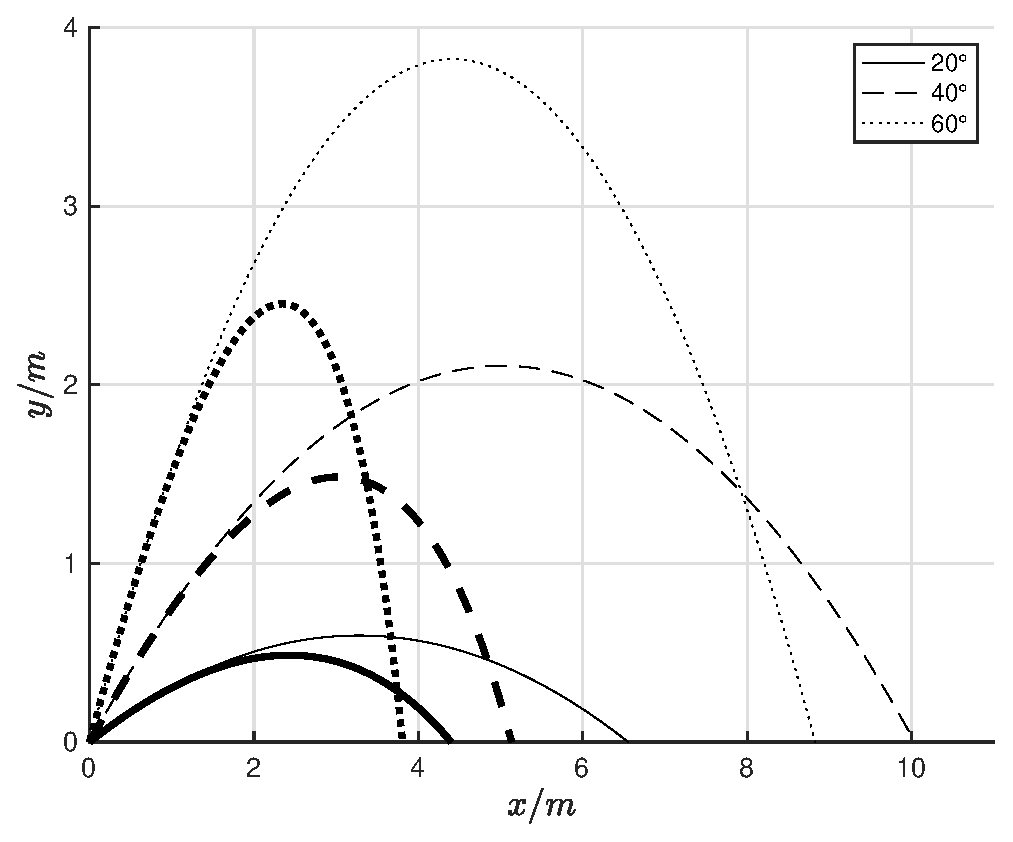
\includegraphics[scale=0.5]{Resources/Graphics/fig2.eps}
    \caption{Kastparabler för vinklarna 20\degree, 40\degree och 60 \degree. Tunna kurvor representerar kaströrelse utan luftmotstånd och tjocka kurvor kaströrelse med luftmotstånd. Föremålets starthastighet är 10 m/s och $k = 1$.}
    \label{fig:2}
\end{figure}

\subsection*{Diskussion}
Till skillnad mot fallet med försummat luftmotstånd är kastparablerna för fallet med luftmotstånd icke-symmetriska. Anledningen till detta är att accelerationen varierar med hastigheten.

En annan observation av resultatet är att föremålet färdas en kortare sträcka i både x-led och y-led i luft än i vakuum. Att föremålets maxhöjd blir mindre i luft beror på att den bromsande kraften i y-led på föremålet på vägen upp är större i luft än i vakuum eftersom accelerationen orsakad av luftmotståndet är riktad åt samma håll som tyngdaccelerationen. Att föremålet färdas en kortare sträcka i horisontalplanet beror på att luftmotståndet bromsar upp rörelsen i x-led men också på att föremålet, till följd av en mindre maxhöjd, befinner sig kortare tid i luften.

Vad beträffar kastvinkeln visar resultatet bland annat att maxhöjden är större desto större kastvinkeln är, vilket förklaras av att hastigheten i y-led blir större med större vinkel, vilket i sin tur betyder att det tar längre tid att bromsa upp rörelsen i y-led. Resultatet visar också, i fallet utan luftmotstånd, att den vinkel som är närmast 45\degree också har längst räckvidd. I fallet med luftmotstånd verkar den optimala kastvinkeln för räckvidden vara något mindre än 45\degree. Detta eftersom räckvidden för vinkeln 20\degree ligger närmare räckvidden för vinkeln 40\degree (vilket är den av de tre vinklar som ligger närmast 45\degree) i fallet med luftmotstånd jämfört med fallet i vakuum.

\subsection*{Referenser}
Mosca, Gene; Tipler, A., Paul. 2008. \textit{Physics for Scientists and Engineers}. 6:e upplagan. W.H. Freeman and Company, New York.

\np
\subsection*{MatLab-kod}
\lstinputlisting[caption={\quad},firstline=2] {Resources/Code/2.m}





